\subsection*{1.1 Definition Strom}

\begin{itemize}
    \item Ladungen mit gleichem Vorzeichen stossen sich ab.
    \item zwei unendlich lange parallele Drähte im Abstand 1 m voneinander, die von einem Strom von 1 A gleichsinnig durchflossen werden, ziehen sich mit einer Kraft von $2 \cdot 10^{-7} N$ pro Meter Leiterlänge an.
    \item Elementarladung: $e = 1.602 \cdot 10^{-19}$
\end{itemize}


Stromstärke: \mathbox{I = \frac{dQ}{dt}}
Ladung: \mathbox{Q = \int\limits_{\Delta t} I dt}
Widerstand: \mathbox{R = \frac{U}{I}, I \sim U}

\begin{tabular}{c c}
    Ohmsche Leiter & nicht-ohmsche Leiter \\
    $I = \frac{U}{R}$ & $R_{\text{diff}} = \frac{dU}{dI}$\\
    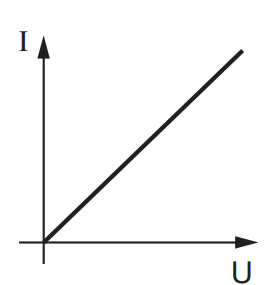
\includegraphics[width = 30mm]{src/images/plot_ohmscher_leiter.png} & 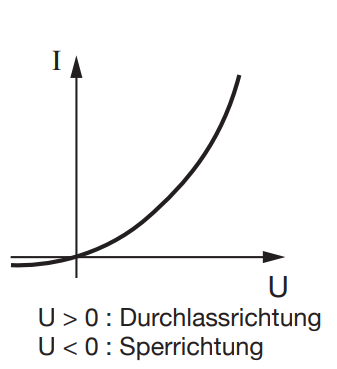
\includegraphics[width = 30mm]{src/images/plot_nicht-ohmscher_leiter.png}
\end{tabular}

